\subsection{Mô hình AdaBoost}

\subsubsection{Mô hình cho tập dữ liệu chỉ bao gồm các quan sát có cột "emailtotal" không phải giá trị null}

\begin{enumerate}[label=(\alph*)]
    \item Đầu vào mô hình là vector thu được từ phân tích thành phần chính sử dụng thuật toán PCA
    
    Ta có bảng kết quả huấn luyện mô hình:

    \begin{python}
                    precision    recall  f1-score   support

   Keeping house       0.13      0.16      0.14        58
           Other       0.00      0.00      0.00         8
         Retired       0.21      0.20      0.20       109
          School       0.00      0.00      0.00        14
Temp not working       0.00      0.00      0.00        15
Unempl, laid off       0.00      0.00      0.00        25
Working fulltime       0.53      0.55      0.54       351
Working parttime       0.11      0.14      0.12        80

        accuracy                           0.35       660
       macro avg       0.12      0.13      0.13       660
    weighted avg       0.34      0.35      0.35       660

    \end{python}

    và ma trận nhầm lẫn:

    \begin{figure}[H]
        \centering
        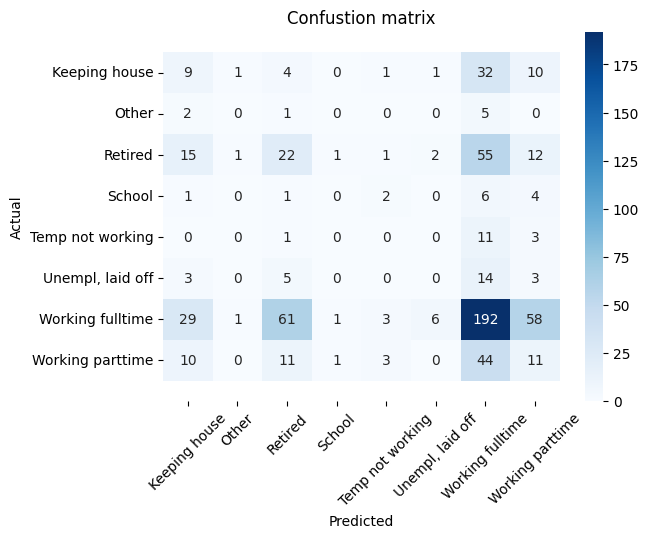
\includegraphics[width=0.6\textwidth]{figures/Thanh/Models/AdaBoost/Non_null_models_confusion_matrix_AdaBoost_PCA_features.png}
        \caption{Ma trận nhầm lẫn của mô hình AdaBoost với vector đầu vào là vector thu được từ phân tích thành phần chính sử dụng thuật toán PCA}
        \label{fig:Non_null_models_confusion_matrix_AdaBoost_PCA_features}
    \end{figure}

    Ta nhận thấy kết quả tuy độ chính xác không cao như hai mô hình Multinomial Logistic Regression và mô hình Random Forest.
    Nhưng một số lớp như Keeping House và Working parttime đã tăng độ hồi tưởng.
    Nhưng vì phân phối của các thành phần chính tương ứng với các nhóm trong cột wrkstat gần như cùng hình dạng, trộn lẫn vào nhau nên việc tăng độ hồi tưởng của các làm khác làm giảm đi khả năng phân loại của lớp nhiều nhất là lớp làm việc toàn thời gian.
    
    Ta sẽ phân tích ngược trở lại trọng số của các tham số tương ứng với các đặc trưng của vector ban đầu từ các tham số ứng với các đặc trưng của các thành phần chính:

    \begin{figure}[H]
        \centering
        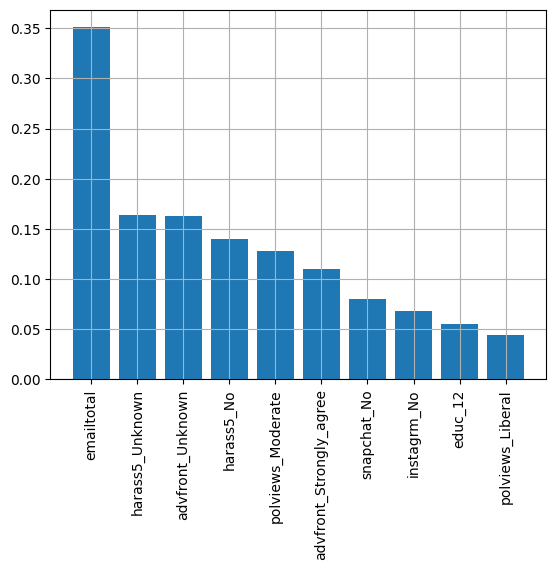
\includegraphics[width=0.6\textwidth]{figures/Thanh/Models/AdaBoost/Non_null_models_Feature_Importance_AdaBoost_PCA_features.png}
        \caption{Biểu đồ cột sắp xếp độ lớn giảm dần (trị tuyệt đối) tham số của các đặc trưng ứng với từng nhãn giả (mô hình với vector đầu vào là vector được phân tích thành phần chính sử dụng thuật toán PCA}
        \label{fig:Non_null_models_Feature_Importance_AdaBoost_PCA_features}
    \end{figure}

    Ta có biểu đồ cột sắp xếp độ lớn giảm dần (trị tuyệt đối) tham số của các đặc trưng ứng với từng nhãn giả thể hiện ở hình \ref{fig:Non_null_models_Feature_Importance_AdaBoost_PCA_features}.
    Ta nhận thấy các cột có trọng số lớn và ảnh hưởng nhiều tới các các nhãn đầu ra là emailtotal, harass5\_Unknown.
    Hai đặc trưng này có tần suất xuất hiện lớn trong tập dữ liệu.

    \item Vector đầu vào là vector gốc ban đầu
    
    Ta có bảng kết quả huấn luyện mô hình:

    \begin{python}
                    precision    recall  f1-score   support

   Keeping house       0.11      0.12      0.11        58
           Other       0.00      0.00      0.00         8
         Retired       0.23      0.20      0.21       109
          School       0.05      0.07      0.06        14
Temp not working       0.00      0.00      0.00        15
Unempl, laid off       0.00      0.00      0.00        25
Working fulltime       0.56      0.55      0.55       351
Working parttime       0.15      0.20      0.17        80

        accuracy                           0.36       660
       macro avg       0.14      0.14      0.14       660
    weighted avg       0.36      0.36      0.36       660
    \end{python}

    và ma trận nhầm lẫn:

    \begin{figure}[H]
        \centering
        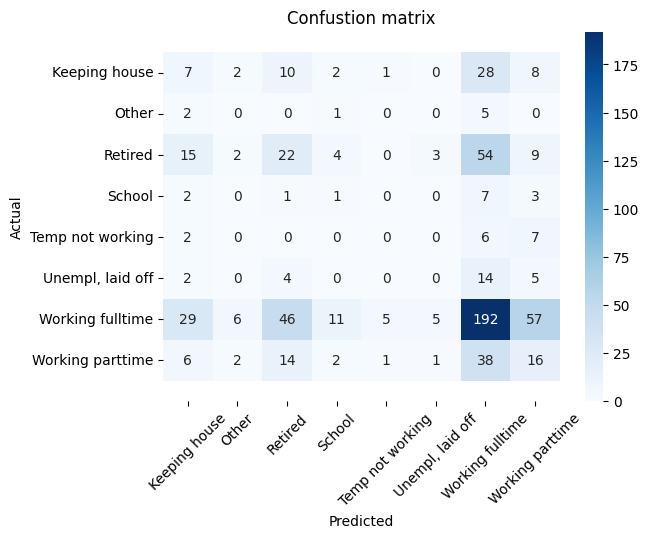
\includegraphics[width=0.6\textwidth]{figures/Thanh/Models/AdaBoost/Non_null_models_confusion_matrix_AdaBoost_original_features.png}
        \caption{Ma trận nhầm lẫn của mô hình AdaBoost khi vector đầu vào là vector gốc ban đầu}
        \label{fig:Non_null_models_confusion_matrix_AdaBoost_original_features}
    \end{figure}
    
    Ta nhận thấy kết quả phân loại không khác nhiều so với trường hợp đầu vào mô hình là vector được phân tích thành phần chính sử dụng thuật toán PCA.
    Ngoại trừ kết quả của nhãn Working parttime tăng lên và lớp Keeping House giảm đi.
    Điều này càng phản ánh sự trỗn lẫn, khó phân biệt của phân phối dữ liệu tương ứng với từng nhãn trong cột wrkstat.

    Ta sẽ phân tích ngược trở lại trọng số của các tham số tương ứng với các đặc trưng của vector ban đầu từ các tham số ứng với các đặc trưng:

    \begin{figure}[H]
        \centering
        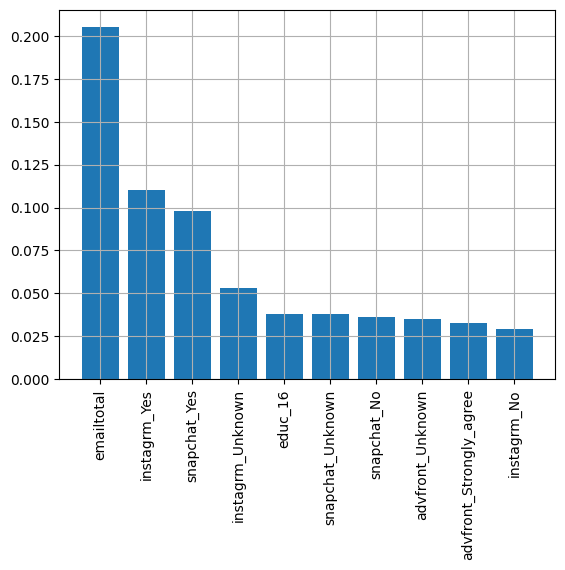
\includegraphics[width=0.6\textwidth]{figures/Thanh/Models/Random_Forest/Non_null_models_Feature_Importance_Random_Forest_original_features.png}
        \caption{Biểu đồ cột sắp xếp độ lớn giảm dần (trị tuyệt đối) tham số của các đặc trưng ứng với từng nhãn giả (mô hình với vector đầu vào là vector gốc ban đầu)}
        \label{fig:Non_null_models_Feature_Importance_Random_Forest_original_features}
    \end{figure}

    Ta có biểu đồ cột sắp xếp độ lớn giảm dần (trị tuyệt đối) của các đặc trưng ứng với từng nhãn giả thể hiện ở hình \ref{fig:Non_null_models_Feature_Importance_Random_Forest_original_features}.
    Ta nhận thấy các đặc trưng có trọng số lớn là polviews\_Liberal, educ\_12 đa số là các đặc trưng ít xuất hiện trong tập dữ liệu.
    emailtotal có trọng số lớn nhất.
\end{enumerate}